\documentclass[11pt]{article}
\usepackage[margin=1in]{geometry}
\usepackage[T1]{fontenc}
\usepackage{amsmath,amssymb,amsthm}
\usepackage{graphicx}
\usepackage{booktabs,tabularx,longtable,array,multirow}
\usepackage{xcolor}
\usepackage{tikz}
\usetikzlibrary{arrows.meta,positioning,calc,fit,backgrounds}
\usepackage[numbers,sort&compress]{natbib}
\usepackage[hidelinks]{hyperref}
\usepackage{xurl}
\usepackage{enumitem}
\usepackage{caption}
\usepackage{adjustbox}
\usepackage[section]{placeins}
\usepackage[ruled,vlined,linesnumbered]{algorithm2e}
\usepackage[most]{tcolorbox}
\definecolor{nb}{HTML}{2A78D6}\definecolor{sb}{HTML}{EB6834}\definecolor{single}{HTML}{D6962C}
\definecolor{ink}{HTML}{1D2622}\definecolor{muted}{HTML}{6B736E}\definecolor{acc}{HTML}{0F6E66}
\newtcolorbox{keybox}[1]{colback=acc!5,colframe=acc!60,fonttitle=\bfseries,title=#1,boxrule=0.6pt,arc=2pt}
\setlist{itemsep=2pt,topsep=4pt}
\captionsetup{font=small,labelfont=bf}
\newcolumntype{L}{>{\raggedright\arraybackslash}X}
\graphicspath{{figures/}}
\newtheorem{proposition}{Proposition}
\SetKwComment{Com}{$\triangleright$\ }{}
\newcommand{\R}{\mathbb{R}}\newcommand{\Z}{\mathbb{Z}}

\title{River LINE Schedule Optimization:\\
\large Technical Report on Data, Optimization Models, Simulation, and Results}
\author{ISE Senior Design Team 22 \quad Client: NJ TRANSIT \quad Faculty advisor: R.~Hildebrand\\
Grado Department of Industrial and Systems Engineering, Virginia Tech}
\date{September 28, 2026}

\begin{document}
\maketitle

\begin{abstract}
NJ TRANSIT's River LINE is a 34-mile diesel light rail line between Camden and Trenton, New Jersey, with seven single-track sections and a 20-car fleet built in 2002--03. Its one weekday timetable needs eight trains at the peaks. When fewer cars pass the morning inspection, trips are cancelled without a plan, and on single track a late train delays the opposing trains it is scheduled to meet. This report documents everything behind our recommendations: the public data and how we processed them, the calibration of a track model to NJ TRANSIT's own timetable, two mixed-integer programs for single-track timetabling (a uniform-headway model and a cyclic pattern model with robustness parameters), a delay-propagation simulation, a fleet simulation with breakdowns and rescues, a combined performance measure, the policies compared, validation against 2024--26 observations, and a bottleneck analysis.

The main results are these. Today's timetable already uses the single track efficiently: its 15/15/30-minute peak fits eight trains into a 150-minute cycle, while an evenly spaced 20-minute service would need nine. Evening out the gaps with the same eight trains (T8) removes the slack at meets and lowers on-time performance from 82\% to 69\% in 2024--25 conditions. A robust eight-train timetable (B8: 160-minute cycle, at least 2.5 minutes of spare time at every meet, layovers of at least 9 minutes) uses the same train-hours and raises on-time performance to 88\%. On our headline measure, reliable trip-miles delivered, B8 adds 3--4 points in every calibrated scenario. Fleet reliability matters more: the change from 2024--25 to 2026 conditions is worth 13--18 points for every plan. Choosing the day's timetable from the 6\,am car count adds about one point in crisis conditions and mainly makes short days predictable. The largest single source of knock-on delay today is the Route~73--Palmyra single-track section.
\end{abstract}

\tableofcontents
\newpage

%======================================================================
\section{Introduction}\label{sec:intro}
\subsection{The client and the line}
The River LINE opened in March 2004 on a former freight line along the Delaware River. It has 21 stations over 33.6 miles between the Entertainment Center in Camden and the Trenton Transit Center, and it connects to PATCO and NJ TRANSIT buses at Walter Rand in Camden, the Atlantic City Line at Pennsauken, and the Northeast Corridor, Amtrak and SEPTA at Trenton. Freight trains use the line at night, so passenger service runs from about 6\,am to 10\,pm \citep{njdot2021riverline}. NJ TRANSIT took over operations from its contractor, Alstom, on February 14, 2026; Kinkisharyo maintains the fleet \citep{njt2025board,ols2027njt}.

The fleet is 20 Stadler GTW diesel cars. Mean distance between failures (MDBF) fell from about 22{,}000 miles in 2021--22 to 2{,}377 in September 2025 and is about 3{,}600 in 2026 \citep{njt_mdbf}. On-time performance was 80--87\% in 2023--25, against 97--99\% on NJ TRANSIT's other light rail lines, and has stayed above 93\% since the takeover \citep{njtod2025,ols2027njt}.

\subsection{Problem statement}\label{sec:problem}
River LINE riders do not receive the service the timetable promises. Three mechanisms cause the loss:
\begin{enumerate}
\item \textbf{Late trains spread.} Opposing trains can pass only on double track. A late train holds every opposing train due to meet it, and those trains are then late for their next meets.
\item \textbf{One plan for every day.} The single published weekday timetable needs eight trains. With fewer serviceable cars, the shortfall appears as unplanned cancellations.
\item \textbf{An unreliable fleet.} Each in-service failure ties up a second car to rescue it and, on single track, blocks both directions.
\end{enumerate}
Our model puts the combined loss at about 31\% of scheduled trip-miles in 2024--25 conditions and 16\% in 2026 conditions (Section~\ref{sec:resrtd}).

\subsection{Objectives, requirements and scope}\label{sec:objectives}
The client asked for a way to choose the day's schedule from the number of cars on the 6\,am hold sheet, weighing on-time performance, frequency and rider impact. We translated this into measurable objectives, with targets still to be agreed with NJ TRANSIT:
\begin{enumerate}[label=O\arabic*.]
\item Reliable trip-miles delivered (Section~\ref{sec:rtd}) of at least 90\%.
\item At least 95\% of trips run arrive on time (NJ TRANSIT's goal is 97\%).
\item Unplanned cancellations of at most 1\% of scheduled trips.
\item No longer peak gaps than today (30 minutes) and no more than today's 109 train-hours per weekday.
\end{enumerate}
\textbf{Requirements.} Every meet must be on double track; the freight window must be kept; tools must use open-source solvers so NJ TRANSIT can run them without academic licenses; results must be reproducible with NJ TRANSIT's own data when it becomes available.
\textbf{In scope:} weekday timetables, the daily plan by car count, delay and fleet simulation, fleet reliability requirements. \textbf{Out of scope:} weekends and special events, crew rostering, bus bridges, fares, and the design of new track.

\subsection{Research questions}
\begin{enumerate}[label=Q\arabic*.]
\item Which timetables fit the single track, and how many trains does each need?
\item How punctual is each timetable when running times vary and incidents occur?
\item Should NJ TRANSIT publish one timetable, or choose one each morning from the car count?
\item Where and when does delay build up, and which levers (timetable, fleet, repairs, dispatching, infrastructure) move performance most?
\end{enumerate}

\subsection{Approach and design methodology}\label{sec:method}
We followed a model-based design cycle: collect data, build a validated representation of the line, generate candidate timetables with optimization, evaluate them by simulation, compare alternatives on one measure, and iterate. Figure~\ref{fig:pipeline} shows how the models connect. The method suits this problem because timetables can be tested only virtually: NJ TRANSIT cannot trial a new schedule without publishing it. The alternatives we considered, and why we kept or dropped them, are summarized in Section~\ref{sec:alts}.

\begin{figure}[ht]\centering
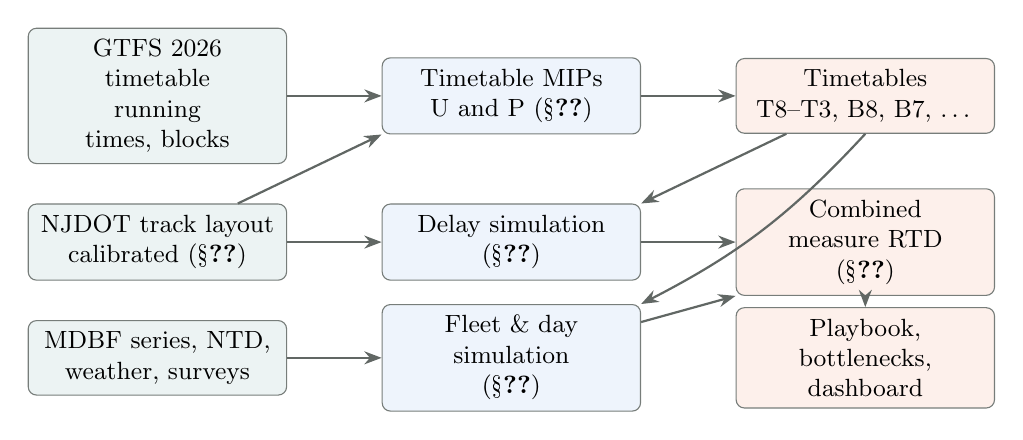
\begin{tikzpicture}[font=\small, node distance=5mm and 7mm,
  box/.style={draw=ink!60, rounded corners=3pt, align=center, inner sep=4pt, fill=white, text width=3.0cm},
  data/.style={box, fill=acc!8}, model/.style={box, fill=nb!8}, outb/.style={box, fill=sb!10},
  arr/.style={-{Stealth[length=2.2mm]}, thick, ink!70}]
\node[data] (gtfs) {GTFS 2026 timetable\\ running times, blocks};
\node[data, below=of gtfs] (track) {NJDOT track layout\\ calibrated (\S\ref{sec:calib})};
\node[data, below=of track] (fleet) {MDBF series, NTD,\\ weather, surveys};
\node[model, right=12mm of gtfs] (mip) {Timetable MIPs\\ U and P (\S\ref{sec:mips})};
\node[model, right=12mm of track] (delay) {Delay simulation\\ (\S\ref{sec:delay})};
\node[model, right=12mm of fleet] (fsim) {Fleet \& day simulation\\ (\S\ref{sec:fleet})};
\node[outb, right=12mm of mip] (tts) {Timetables\\ T8--T3, B8, B7, \dots};
\node[outb, right=12mm of delay] (rtd) {Combined measure RTD\\ (\S\ref{sec:rtd})};
\node[outb, right=12mm of fsim] (pb) {Playbook, bottlenecks,\\ dashboard};
\draw[arr] (gtfs) -- (mip); \draw[arr] (track) -- (mip.south west);
\draw[arr] (track) -- (delay); \draw[arr] (fleet) -- (fsim);
\draw[arr] (mip) -- (tts); \draw[arr] (tts) -- (delay.north east); \draw[arr] (tts.south) to[bend left=10] (fsim.north east);
\draw[arr] (delay) -- (rtd); \draw[arr] (fsim) -- (rtd.south west); \draw[arr] (rtd) -- (pb);
\end{tikzpicture}
\caption{Data (green), models (blue) and outputs (orange).}\label{fig:pipeline}
\end{figure}

%======================================================================
\section{Data}\label{sec:data}
\subsection{Sources}
Table~\ref{tab:data} lists the data. All are public; the data request in the companion materials lists what only NJ TRANSIT can provide (hold sheets, failure and work-order logs, train-level arrival and cancellation records, the official track chart).

\begin{table}[ht]\centering\small
\begin{tabularx}{\textwidth}{@{}p{3.6cm}Lp{2.6cm}@{}}
\toprule
Data & Used for & Source \\ \midrule
GTFS schedule, Sept.~2026 & 87 weekday trips; times at 21 stations; 12 vehicle blocks; station-to-station running times & \citet{njt2026gtfs} \\
GTFS schedule, 2014 & Track shape (33.6 mi); running-time comparison & \citet{njt2014gtfs} \\
NJDOT SSO Appendix F & Single/double track by milepost; sidings; yards (Burlington 2 cars, Trenton 8) & \citet{njdot2021riverline} \\
OpenStreetMap & Posted speeds; cross-check of single track & \citet{osm2026} \\
NJ TRANSIT MDBF series & Monthly River LINE miles between failures, 2017--2026 & \citet{njt_mdbf} \\
NTD (mode YR, ID 20080) & Ridership, failures, vehicles in service, cost per revenue hour & \citet{ntd_monthly,ntd_ts21,ntd_breakdowns2224} \\
NOAA GHCN-Daily, Trenton & Hot days per summer (21 on average at $\ge$90\textdegree F) & \citet{noaa_ghcnd} \\
NJ OLS budget analyses; press & On-time performance 2023--26; worst days; events & \citet{ols2027njt,news12_2025,njtod2026} \\
DVRPC on-board survey & Trip purpose (63\% work), car availability & \citet{dvrpc2013riverline} \\
\bottomrule
\end{tabularx}
\caption{Public data used.}\label{tab:data}
\end{table}

\subsection{Processing}
\begin{itemize}
\item \textbf{Line geometry.} Station positions are distances along the 2014 GTFS shape, measured from the Entertainment Center, $x_1=0,\dots,x_{21}=33.59$ miles.
\item \textbf{Running times.} For each direction and each pair of consecutive stations we take the median scheduled time over all 2026 weekday trips. Cumulative sums give the northbound clock $\tau^N(x)$ and southbound clock $\tau^S(x)$, interpolated linearly between stations. Both directions take 67 minutes end to end, unchanged since 2014; at posted speeds with no stops the trip would take 46 minutes.
\item \textbf{Blocks.} GTFS block identifiers give NJ TRANSIT's vehicle duties: 8 trains at the peaks and 6 midday, 108.9 train-hours.
\item \textbf{Failure rates.} The NJ TRANSIT monthly MDBF series averages 3{,}661 miles in 2024--25 and 3{,}568 in March--August 2026. Its 2022 and 2024 annual means (22{,}337 and 4{,}192) match the press figures, so we treat it as the authoritative series (Figure~\ref{fig:mdbf}).
\item \textbf{Cost.} We use \$547 per train-hour: NTD FY2024 vehicle operations plus vehicle maintenance (\$20.9M) divided by 38{,}212 vehicle revenue hours \citep{ntd_ts21}. The full average of \$952 includes costs that do not vary with service.
\end{itemize}

\begin{figure}[ht]\centering
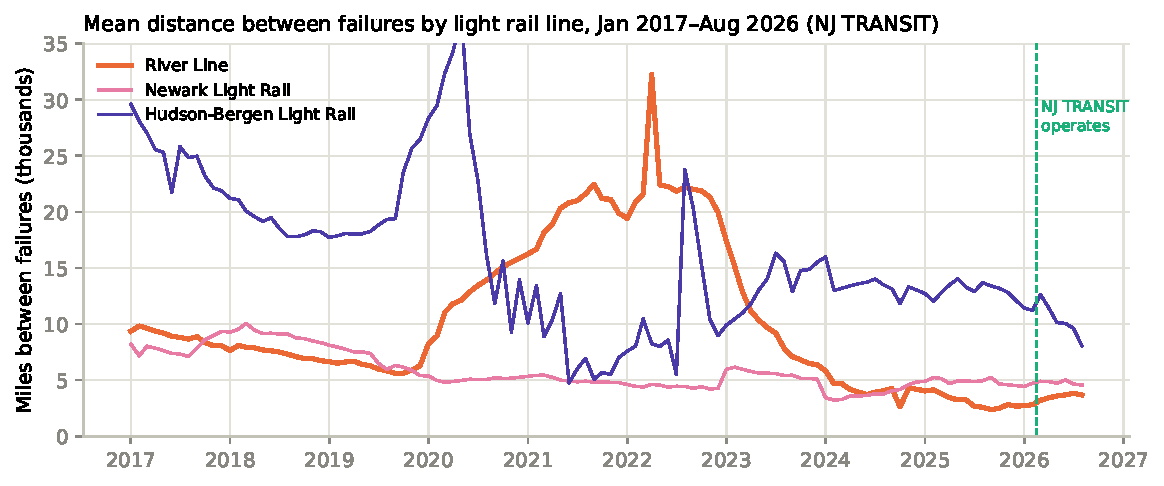
\includegraphics[width=0.9\textwidth]{fig_ctx_mdbf.pdf}
\caption{River LINE mean distance between failures, monthly, from NJ TRANSIT's published series \citep{njt_mdbf}.}\label{fig:mdbf}
\end{figure}

\subsection{Calibrating the track model}\label{sec:calib}
A timetable is feasible only if opposing trains pass on double track, so the positions of the single-track sections matter more than any other input. NJDOT publishes them by freight milepost, which does not map directly to the passenger track distance.

\paragraph{Method.} We located every scheduled meet in NJ TRANSIT's 2026 timetable (213 crossings of a northbound and a southbound trip), mapped NJDOT mileposts onto track distance by linear scaling, and counted meets that fall on single track. We then fitted a shift $\delta$ applied north of milepost $m_0$ and ramped over $\Delta$ miles:
\[x(\text{mp}) = s\cdot\text{mp} + \delta\cdot\min\{1,\max\{0,(\text{mp}-m_0)/\Delta\}\},\]
where $s$ rescales mileposts to the shape length. The fit is $\delta=1.5$, $m_0=12$, $\Delta=2$.

\paragraph{Result.} Scaled NJDOT mileposts put 61 scheduled meets on single track. The calibrated layout leaves one, at the edge of the Pennsauken siding (Figure~\ref{fig:meets}); any shift between 1.3 and 1.8 miles works. The seven calibrated single-track sections are listed in Table~\ref{tab:sections}. This is an assumption until NJ TRANSIT provides its track chart; all timetables can be re-solved in minutes once it does.

\begin{figure}[ht]\centering
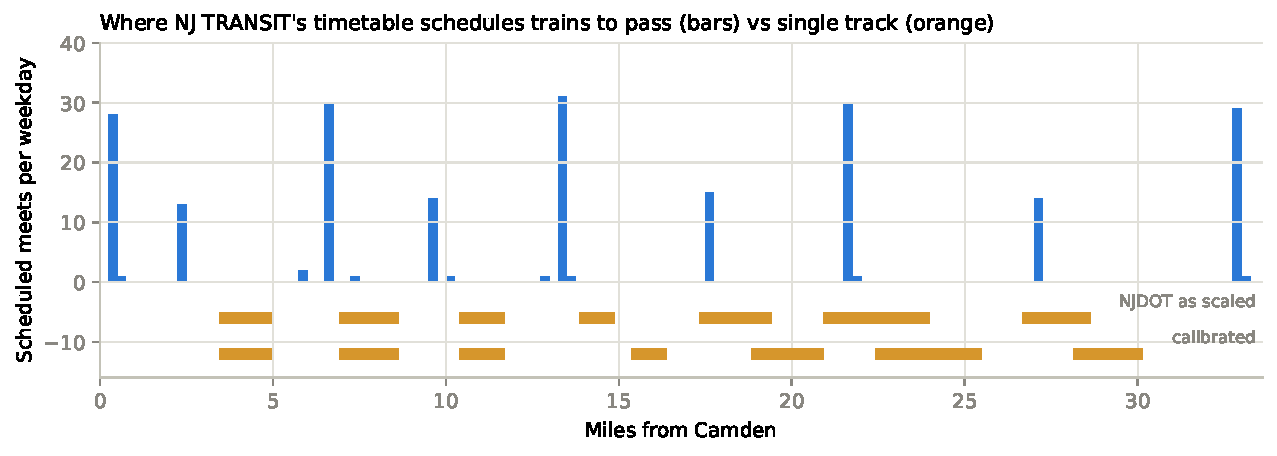
\includegraphics[width=\textwidth]{fig_meets_calibration.pdf}
\caption{Where the September 2026 timetable schedules meets (bars), against single track before and after calibration (orange).}\label{fig:meets}
\end{figure}

\begin{table}[ht]\centering\small
\begin{adjustbox}{max width=\linewidth}
\begin{tabular}{@{}clrrrl@{}}
\toprule
$s$ & Section & From (mi) & To (mi) & Crossing time (min) & Stations on the single track \\ \midrule
1 & 36th Street & 3.47 & 4.95 & 2.8 & 36th Street \\
2 & Route 73 -- Palmyra & 6.94 & 8.62 & 4.5 & Pennsauken--Route 73, Palmyra \\
3 & Cinnaminson -- Riverside & 10.40 & 11.69 & 2.4 & -- \\
4 & Beverly -- Burlington South & 15.37 & 16.36 & 1.5 & -- \\
5 & Burlington -- Florence & 18.84 & 20.92 & 3.2 & -- \\
6 & Roebling & 22.41 & 25.48 & 4.1 & Roebling \\
7 & Bordentown -- Cass Street & 28.15 & 30.14 & 2.7 & -- \\
\bottomrule
\end{tabular}
\end{adjustbox}
\caption{Calibrated single-track sections. Crossing time is the median scheduled time for a train to traverse the section in today's timetable.}\label{tab:sections}
\end{table}

\subsection{Data limitations}
\begin{itemize}
\item No public train-level records: on-time performance and cancellations are available only as monthly or annual figures and press reports.
\item No public repair times or hold sheets: fleet availability is inferred (Section~\ref{sec:calibinputs}).
\item No ridership by hour: waiting-time measures use an assumed hourly profile.
\item The public on-time file combines all light rail lines; River LINE figures come from budget analyses and press.
\end{itemize}

%======================================================================
\section{Notation and single-track representation}\label{sec:notation}
The line is divided into sections $\mathcal{S}$ (single track) and $\mathcal{D}$ (double track, where trains may pass and wait). For single-track section $s=[\alpha_s,\beta_s]$ the northbound and southbound occupation times are
\[o^N_s=\tau^N(\beta_s)-\tau^N(\alpha_s),\qquad o^S_s=\tau^S(\alpha_s)-\tau^S(\beta_s).\]
A northbound train enters $s$ at $\alpha_s$ and a southbound train at $\beta_s$. Two opposing trains may not occupy $s$ at the same time; a clearance buffer $g$ separates them. Table~\ref{tab:notation} collects the notation used in the optimization models.

\begin{table}[ht]\centering\small
\begin{tabularx}{\textwidth}{@{}lL@{}}
\toprule
Symbol & Meaning \\ \midrule
$K$ & number of trains in the cyclic pattern \\
$C$ & cycle length (minutes); each train makes one round trip per cycle \\
$T$ & headway of a uniform timetable (minutes) \\
$R^N, R^S$ & scheduled running time Camden$\to$Trenton and Trenton$\to$Camden (67 min each) \\
$o^N_s, o^S_s$ & occupation times of single-track section $s$ \\
$g$ & clearance buffer at single-track hand-offs (0.5 min nominal; 2.5 in B8/B7) \\
$\ell_{\min}^T,\ell_{\min}^C$ & minimum layover at Trenton and Camden \\
$h_{\min}$ & minimum separation of consecutive departures (6 min) \\
$a_k, b_k$ & departure of train $k$ from Camden and from Trenton within the cycle \\
$w^N_{kd}, w^S_{kd}$ & extra wait of train $k$ at double-track section $d$ \\
$\ell^T_k$ & layover of train $k$ at Trenton \\
$z_{ijs}\in\Z$ & periodic offset integer for northbound train $i$, southbound train $j$, section $s$ \\
\bottomrule
\end{tabularx}
\caption{Notation.}\label{tab:notation}
\end{table}

%======================================================================
\section{Optimization models}\label{sec:mips}
Both models are periodic event scheduling problems (PESP) \citep{serafini1989mathematical,liebchen2008first}. The core constraint says that, modulo the period, a southbound entry into a single-track section must fall in the window when the section is free of northbound trains.

\subsection{Model U: uniform-headway timetables}\label{sec:modelU}
For a headway $T$, northbound trains leave Camden at $0,T,2T,\dots$ and southbound trains leave Trenton at $\phi+nT$. Let $s^N_d,s^S_d\in[0,\bar w]$ be waits at double-track section $d$ (identical for every train, since the timetable is periodic with period $T$), $m_T,m_C\in\Z_+$ the numbers of headways spent between departures at each end, and $z_s\in\Z$. Define the entry times
\[p_s=\tau^N(\alpha_s)+\sum_{d:\,\beta_d\le\alpha_s}s^N_d,\qquad q_s=\phi+\tau^S(\beta_s)+\sum_{d:\,\alpha_d\ge\beta_s}s^S_d.\]
Model U is
\begin{align}
\min\quad & 1000\,m_C+\textstyle\sum_d (s^N_d+s^S_d) \label{eq:U-obj}\\
\text{s.t.}\quad & 0\;\le\; q_s-p_s-o^N_s-g+T z_s\;\le\; T-o^N_s-o^S_s-2g && \forall s\in\mathcal{S} \label{eq:U-pesp}\\
& \ell_{\min}\le \phi+Tm_T-\bigl(R^N+\textstyle\sum_d s^N_d\bigr)\le \ell_{\min}+T && \text{(Trenton layover)} \\
& Tm_C-\bigl(\phi+Tm_T+R^S+\textstyle\sum_d s^S_d\bigr)\ge \ell_{\min} && \text{(Camden layover)} \\
& 0\le\phi<T,\ 0\le s^N_d,s^S_d\le\bar w,\ m_T,m_C,z_s\in\Z.
\end{align}
The round trip takes $Tm_C$ minutes, so $m_C$ is the number of trains; the weight 1000 makes the objective lexicographic (fewest trains, then least added waiting). Constraint \eqref{eq:U-pesp} is the standard PESP linearization of $(q_s-p_s-o^N_s-g)\bmod T\in[0,\,T-o^N_s-o^S_s-2g]$: the southbound train enters after the northbound train has cleared, and leaves before the next northbound train arrives. A necessary condition for feasibility is $T\ge \max_s(o^N_s+o^S_s+2g)$.

We solve Model U for every $T\in\{12,\dots,60\}$ with HiGHS through PuLP; each instance solves in under a second.

\subsection{Model P: cyclic pattern timetables}\label{sec:modelP}
A uniform headway wastes trains whenever the round trip is not a multiple of $T$. Model P fixes $K$ and $C$ and lets each train's departure $a_k$ vary, so gaps may differ, as in NJ TRANSIT's 15/15/30.

\paragraph{Variables.} $a_k\in[0,C]$; $w^N_{kd},w^S_{kd}\in[\underline{w}_d,\,\underline{w}_d+\bar w]$ where $\underline w_d$ is an optional scheduled hold; $\ell^T_k\ge\ell^T_{\min}$; $z_{ijs}\in\{-4,\dots,4\}$; epigraph variables $u$ for the squared gaps.
\paragraph{Derived times.} Southbound departure from Trenton and the entry times into section $s$:
\begin{align*}
b_k&=a_k+R^N+\textstyle\sum_d w^N_{kd}+\ell^T_k,\\
p_{is}&=a_i+\tau^N(\alpha_s)+\textstyle\sum_{d:\,\beta_d\le\alpha_s}w^N_{id},\qquad
q_{js}=b_j+\tau^S(\beta_s)+\textstyle\sum_{d:\,\alpha_d\ge\beta_s}w^S_{jd}.
\end{align*}
\paragraph{Constraints.}
\begin{align}
& a_0=0,\quad a_{k+1}-a_k\ge h_{\min}\ (k<K-1),\quad C-a_{K-1}\ge h_{\min} && \text{(order, symmetry)}\label{eq:P-order}\\
& b_{k+1}-b_k\ge h_{\min},\quad b_0+C-b_{K-1}\ge h_{\min} && \text{(Trenton spacing)}\\
& a_k+C-\bigl(b_k+R^S+\textstyle\sum_d w^S_{kd}\bigr)\ge \ell^C_{\min} && \forall k\ \text{(cycle closes)}\label{eq:P-cycle}\\
& 0\le q_{js}-p_{is}-o^N_s-g+Cz_{ijs}\le C-o^N_s-o^S_s-2g && \forall i,j,s \label{eq:P-pesp}
\end{align}
Constraint \eqref{eq:P-cycle} makes the pattern one of $K$ trains each completing a round trip per cycle, so exactly $K$ trains run it. Constraint \eqref{eq:P-pesp} applies the PESP window to every pair of a northbound train $i$ and a southbound train $j$ on every single-track section, so every meet in the repeating pattern falls on double track.

\paragraph{Objective.} Let $\mathcal{G}(x_0,\dots,x_{n-1})=\{x_{t+1}-x_t\}_{t<n-1}\cup\{x_0+C-x_{n-1}\}$ be the cyclic gaps of a set of departure times. The objective is
\begin{equation}\label{eq:P-obj}
\min\ \sum_{\gamma\in\mathcal{G}(a)\cup\mathcal{G}(b)}\gamma^2\;+\;\omega\sum_{\gamma\in\mathcal{G}(a_M)\cup\mathcal{G}(b_M)}\gamma^2\;+\;0.2\sum_{k,d}\bigl(w^N_{kd}+w^S_{kd}-2\underline w_d\bigr),
\end{equation}
where $M\subset\{0,\dots,K-1\}$ is the subset of trains that keep running midday and $\omega=1$. The squared gaps are the timetable's contribution to riders' waiting: with random arrivals the mean wait is
\begin{equation}\label{eq:wait}
\mathbb{E}[W]=\frac{\sum_t\gamma_t^2}{2C}=\frac{\mathbb{E}[H]}{2}\bigl(1+\mathrm{CV}^2(H)\bigr)
\end{equation}
\citep{welding1957instability,osuna1972control}, so minimizing $\sum\gamma^2$ with $C$ fixed minimizes mean wait. The last term discourages unnecessary siding waits.

\paragraph{Linearization.} Each $\gamma^2$ is replaced by $u_\gamma\ge 2t\gamma-t^2$ for $t\in\{4,6,\dots,98\}$, the tangent lines of $\gamma^2$ at even integers.
\begin{proposition}
For $\gamma\in[4,98]$, $0\le\gamma^2-\max_t(2t\gamma-t^2)\le 1$.
\end{proposition}
\begin{proof}
$\gamma^2-(2t\gamma-t^2)=(\gamma-t)^2\ge0$, and for $\gamma$ between consecutive tangent points $t$ and $t+2$ the nearest one is within 1, so the minimum over $t$ of $(\gamma-t)^2$ is at most 1.
\end{proof}
Since every gap is at least $h_{\min}=6$ and at most $C$, the linearized objective is within $2K(1+\omega)$ square-minutes of the true one, which is negligible against objective values of about 15{,}000.

\paragraph{Robustness parameters.} Model P has four levers that trade even spacing against punctuality: the buffer $g$ at every hand-off, the minimum layovers $\ell_{\min}^T,\ell_{\min}^C$, the cycle $C$ (a longer cycle leaves more slack for the same $K$), and scheduled holds $\underline w_d$ just before single track. Running times can also be scaled (e.g.\ by 1.06 for a summer timetable with heat speed restrictions).

\paragraph{Size and solution.} For $K=8$ there are $8\times8\times7=448$ integer variables $z_{ijs}$, 896 PESP inequalities, about 110 continuous variables, and $49\times|\text{gaps}|$ tangent cuts. We solve with HiGHS (branch and cut) through PuLP with a time limit of 90--240 seconds. Every pattern used in this report was solved to optimality (HiGHS default gap tolerance) within the limit; runs that stopped at the limit were discarded. Because the midday subset $M$ enters the objective, we solve one instance per subset; subsets that are rotations of each other are equivalent, so we enumerate one representative per rotation class (e.g.\ 5 classes of 6-subsets of 8 trains) in parallel and keep the best.

\subsection{From a pattern to a full-day timetable}\label{sec:build}
Algorithm~\ref{alg:build} turns a pattern into a weekday timetable. Because any subset of a conflict-free pattern is conflict-free, dropping trains off-peak never creates a new conflict. Vehicle blocks are then formed first-in-first-out at each terminal with a minimum turnaround, and an independent conflict checker verifies that no two opposing trips occupy the same single-track section within $g$ of each other.

\begin{algorithm}[ht]
\caption{Build a weekday timetable from pattern $(a,b,w)$}\label{alg:build}
\KwIn{pattern for $K$ trains on cycle $C$; midday subset $M$; peak windows $P=\{[5{:}40,9{:}00],[14{:}15,18{:}30]\}$; service span $[5{:}40,21{:}05]$}
\For{each cycle $n$ and train $k$}{
  $t\gets nC+a_k$ \Com*{northbound departure from Camden}
  \If{$t$ in service span \textbf{and} ($k\in M$ \textbf{or} $t\in P$)}{create northbound trip with station times $t+\tau^N(x)+$waits; create its southbound return at $nC+b_k$}
}
Chain trips into blocks FIFO at each terminal with turnaround $\ge 5$ min\;
Verify with the conflict checker (all pairs, all sections)\;
\end{algorithm}

The midday subset $M$ is chosen with the pattern (it is in the objective); for the T-tiers we chose the $k$-subset with the most even spacing after the fact by enumeration.

\subsection{Timetables produced}\label{sec:tts}
\begin{description}[itemsep=1pt]
\item[T8--T3] Model P with $g=0.5$, 5-minute layovers, $C=150$; one tier per train count (8 to 3).
\item[U8--U4] Model U, one headway per period; conflict-free within periods but not at peak/off-peak changeovers.
\item[E5, E6] Eight peak trains with 5 or 6 midday trains, peak and midday spacing optimized jointly.
\item[R8] $C=160$, 8-minute layovers. \textbf{S8:} 6\% of running time moved into scheduled holds before single track. \textbf{G8:} $g=2$.
\item[W7] Summer: running times $\times1.06$, 7 trains, $C=160$.
\item[B8, B7] Robust: $C=160$, $g=2.5$, $\ell_{\min}=9$, with 8 and 7 trains; chosen from a sweep (Table~\ref{tab:sweep}).
\end{description}

%======================================================================
\section{Delay-propagation simulation}\label{sec:delay}
The optimization models judge a timetable as printed. The delay simulation tests how it behaves when trains run late.

\subsection{Model}
Each trip is a sequence of nodes: stations and the ends of single-track sections. For node $i$ with scheduled departure $d_i$ and scheduled running time $r_i$ to node $i+1$,
\begin{align}
A_{i+1}&=D_i+(1-\sigma)\,r_i\,h\,Y\,X_i+\mathbb{1}[\text{incident at }i]\,E, \label{eq:run}\\
D_i&=\max\bigl\{A_i,\ d_i\cdot\mathbb{1}[i\text{ is a station or hold}],\ \text{Exit}(\text{opposing train due first})+g-\epsilon_i\bigr\}. \label{eq:dep}
\end{align}
Here $\sigma=0.10$ is the running-time supplement (the scheduled time includes 10\% recovery time); $h=1$ on a normal day and $1.06$ on a hot day; $Y\sim\mathrm{LN}(-0.035^2/2,\,0.035)$ is a trip factor and $X_i\sim\mathrm{LN}(-0.12^2/2,\,0.12)$ a segment factor, both with mean 1; incidents (ramp deployments, grade crossings, door faults) occur with probability $p_{\text{inc}}$ per trip at a uniformly chosen node and add $E\sim\mathrm{Exp}(\text{mean }6\text{ min})$. Trains never leave a station early. The third term is the single-track rule: a train may enter a section only after the opposing train scheduled through it just before has left, plus the buffer. The meet order is fixed by the timetable, as a dispatcher normally keeps it \citep{carey1995model,higgins1996optimal}. A train starts its next trip no earlier than 3 minutes after arriving. A trip is on time if it reaches its last stop less than 6 minutes late, NJ TRANSIT's definition \citep{njt2019otp}.

\paragraph{Tolerance for published timetables.} GTFS times are rounded to the minute and the calibrated siding limits are approximate, so a few meets in NJ TRANSIT's timetable are scheduled up to about 3 minutes ``inside'' a single-track section. We take such a scheduled overlap as feasible by allowing $\epsilon_i\le 3$ minutes where the schedule itself requires it; without this, the published timetable would incur knock-on delay even with no randomness.

\subsection{Algorithm}
The simulation advances trains block by block (Algorithm~\ref{alg:delay}). A train that reaches a single-track entrance whose blocking opposing train has not yet left is parked in a waiting list keyed by that train and node, and resumes when it passes. This event-driven scheme needs no global clock and simulates a day of 87 trips in a few milliseconds.

\begin{algorithm}[ht]
\caption{One simulated day of delay propagation}\label{alg:delay}
\KwIn{trips with nodes, scheduled times and blocks; for each single-track entry $(i,k)$ the opposing blocker $(j,k')$ from the scheduled order}
Draw $Y$, $X$, incidents for all trips\;
Push every block onto a stack\;
\While{the stack is not empty}{
  Pop block $b$; let $i$ be its current trip and $k$ its current node\;
  \While{block $b$ has trips left}{
    Compute the earliest departure from node $k$ (station hold, arrival)\;
    \If{$(i,k)$ has a blocker $(j,k')$}{
      \eIf{$(j,k')$ has not been passed}{add $b$ to waiting$[(j,k')]$; \textbf{break}}{$D\gets\max(D,\text{Exit}(j,k')+g-\epsilon)$; record knock-on wait}
    }
    Record $\text{Exit}(i,k)\gets D$; push all blocks in waiting$[(i,k)]$ onto the stack\;
    \eIf{$k$ is the last node}{next trip of $b$ starts at $\max(D+3,\text{scheduled})$}{$A_{k+1}\gets$ \eqref{eq:run}; $k\gets k+1$}
  }
}
\If{blocks remain but all are waiting (inconsistent timetable)}{release the earliest waiting train and continue}
\end{algorithm}

\subsection{Calibration and experiments}
The only fitted parameter is the incident probability $p_{\text{inc}}$. For a target on-time rate we find $p_{\text{inc}}$ by bisection on $[0,0.5]$ (10 steps, 200 simulated days per step, fixed seed) so that today's timetable matches the target:
\begin{itemize}
\item \textbf{2024--25 (Alstom) regime:} target 83\% (NJ TRANSIT reported 80--87\%); $p_{\text{inc}}=0.210$.
\item \textbf{2026 (NJ TRANSIT) regime:} target 93\% (``above 93 percent'' since the takeover); $p_{\text{inc}}=0.110$.
\end{itemize}
Every timetable is then simulated for 300 normal and 300 hot days with common random numbers (the same seeds), so differences between timetables are not sampling noise. We record on-time share, mean lateness, and every knock-on wait with its location and time; the bottleneck analysis (Section~\ref{sec:resbottle}) aggregates the waits by section and hour.

%======================================================================
\section{Fleet and day simulation}\label{sec:fleet}
The fleet simulation is the engine of the dashboard (JavaScript), run headless for experiments. It models what the delay simulation does not: car availability, breakdowns, rescues, and cancellations.

\subsection{One day}
\begin{enumerate}
\item \textbf{Plan.} Given the cars available at 6\,am, $A$, a policy selects the day's timetable and the number of protect (spare) cars held back (Section~\ref{sec:policies}). The timetable's blocks are the vehicle duties.
\item \textbf{Car assignment.} Each block takes a free car at its start, preferring a car coming off another block; with no free car, the block's trips are cancelled.
\item \textbf{Failures.} A car in service fails after an exponential time with rate $\lambda=(2L/150)/\text{MDBF}_{\text{season}}$ per operating minute, where $2L/150$ is car-miles per minute of a train on a 150-minute round trip. Season multipliers on MDBF are 0.85 (winter), 1.25 (spring), 0.65 (summer), 1.0 (fall).
\item \textbf{Rescue.} A failed car is rescued by the nearest protect car (dispatch 10 min, travel at 25 mph, couple 10 min, tow to the nearest yard at 15 mph). With no protect car, the nearest train in service is pulled; its trips are cancelled until the rescue ends, and the failed block is cancelled for the rest of its run. With no car at all, the shop recovers the car after 30 minutes and trips are lost.
\item \textbf{Blockage.} A failure on single track blocks both directions for 35 minutes; trains due through the section are held and become late.
\item \textbf{Background lateness.} Independently of failures, a trip starts 6.5--12.5 minutes late with a seasonal probability (3--9\%).
\end{enumerate}

\subsection{A year}
Algorithm~\ref{alg:year} links days through the repair shop. Repair times are geometric with mean $\bar r$ days; each available car also develops a depot defect with probability 1\% per day; three cars are out long-term (e.g.\ heavy overhaul). A simulated year is 365 days after a 60-day warm-up; we run 10 years per policy and scenario.

\begin{algorithm}[ht]
\caption{One simulated year}\label{alg:year}
Start with half of the available pool in repair\;
\For{day $=1,\dots,425$}{
  Depot defects: each available car enters repair with probability 0.01\;
  $A\gets 20-3-|\text{repair}|$; season from the day of year\;
  Simulate the day under the policy with $A$ cars (Section 6.1)\;
  Each failed car enters repair with a geometric repair time (mean $\bar r$)\;
  Decrement repair times; release finished cars\;
  \If{day $>60$}{record trips scheduled, run, cancelled; trip-miles run; timetable used}
}
\end{algorithm}

%======================================================================
\section{Combined measure, scenarios and policies}\label{sec:rtd}
\subsection{Reliable trip-miles delivered}
Cancellations and lateness are usually reported separately, which lets a plan look good on one while failing on the other. We combine them. For day $t$ with timetable $\pi_t$,
\begin{equation}\label{eq:rtd}
\mathrm{RTD}=\frac{\sum_t \min\{M^{\text{run}}_t,\,M^{\text{base}}\}\cdot \mathrm{OTP}(\pi_t,\text{season}_t)}{\sum_t M^{\text{base}}},
\end{equation}
where $M^{\text{run}}_t$ is the trip-miles run on day $t$ (cancelled trips excluded), $M^{\text{base}}$ the trip-miles in today's timetable, and $\mathrm{OTP}(\pi,\cdot)$ the delay-simulation on-time rate for timetable $\pi$ in the scenario's regime; in summer $\mathrm{OTP}=0.77\,\mathrm{OTP}_{\text{normal}}+0.23\,\mathrm{OTP}_{\text{hot}}$ (21 hot days out of 92). The cap at $M^{\text{base}}$ means that running more miles than today earns no credit. RTD is 100\% only if every trip of today's timetable runs and arrives on time.

\subsection{Calibrated scenarios}\label{sec:calibinputs}
\begin{table}[ht]\centering\small
\begin{adjustbox}{max width=\linewidth}
\begin{tabular}{@{}lrrll@{}}
\toprule
Scenario & MDBF (mi) & Mean repair (days) & Delay regime & Basis \\ \midrule
S1 Alstom era 2024--25 & 3{,}661 & 10 & 83\% & MDBF series; Aug.~2024 interim schedule \\
S2 NJ TRANSIT 2026 & 3{,}568 & 5 & 93\% & MDBF series; NTD 12 cars in service \\
S3 Renewed fleet & 10{,}000 & 5 & 93\% & about the 2017 level \\
\bottomrule
\end{tabular}
\end{adjustbox}
\caption{Scenarios. Repair times are not public; they are inferred so that simulated availability matches observed fleet behavior (Section~\ref{sec:valid}).}\label{tab:scen}
\end{table}

\subsection{Policies}\label{sec:policies}
\begin{enumerate}[label=P\arabic*.]
\item \textbf{Today:} publish NJ TRANSIT's timetable every day; cancel what cannot run.
\item \textbf{B8 every day:} publish B8; cancel what cannot run.
\item \textbf{T-tiers:} with $A$ cars and one protect car, run tier T$\min(8,A-1)$.
\item \textbf{Robust tiers:} as P3 but B8 for 8 trains and B7 for 7 (T6--T3 below).
\item \textbf{Robust tiers + W7} in summer.
\item \textbf{Robust tiers without a protect car.}
\end{enumerate}
The \emph{playbook} is the policy-by-car-count table: for each $A$ and season, the plan with the highest RTD among those that cancel at most 5\% of their own trips, with ties within 0.3 points going to the lower operating cost (300 simulated days per cell).

%======================================================================
\section{Alternatives considered}\label{sec:alts}
\begin{table}[ht]\centering\small
\begin{tabularx}{\textwidth}{@{}p{3.4cm}LL@{}}
\toprule
Alternative & Why considered & Outcome \\ \midrule
Uniform clock-face headways (Model U) & Easy to remember; standard practice & Needs 9 trains for 20-minute peaks; changeovers conflict. Kept as a reference only. \\
Even spacing, same trains (T8) & Shorter waits & Rejected: 69\% on time vs 82\% today. \\
Slack placement variants (S8, R8, G8) & Recover punctuality one lever at a time & Each recovers part of the loss; none matches B8. \\
Robust pattern (B8, B7) & Slack at meets and layovers together & Recommended. \\
Summer timetable (W7) & Heat speed restrictions & Best on hot days, but fewer trips; loses on RTD unless restrictions are confirmed. \\
Daily tiers by car count & Predictable service on short days & Adds $\approx$1 RTD point in S1, none in S2; cuts unplanned cancellations sharply. \\
Microscopic simulation (e.g.\ OpenTrack) & Detailed signalling & Not available without NJ TRANSIT data and licenses; our node-level model is sufficient for meet-level effects. \\
Stochastic two-stage tier selection & Choose which tiers to publish & Future work (Section~\ref{sec:future}). \\
\bottomrule
\end{tabularx}
\caption{Design alternatives and decisions.}\label{tab:alts}
\end{table}

%======================================================================
\section{Results}\label{sec:results}
\subsection{Today's timetable (Q1)}\label{sec:restoday}
NJ TRANSIT's September 2026 timetable has 87 weekday trips on 12 vehicle blocks, 8 trains at the peaks and 6 midday, and 108.9 train-hours (Figure~\ref{fig:gtfs}). Each peak train makes a 150-minute round trip: 67 minutes each way plus about 16 minutes of layovers. Eight trains in 150 minutes average 18.75 minutes apart; NJ TRANSIT spaces them 15, 15 and 30. By \eqref{eq:wait}, the mean morning wait toward Trenton at Walter Rand is 9.6 minutes, against 8.75 for the same trains evenly spaced.

\begin{figure}[ht]\centering
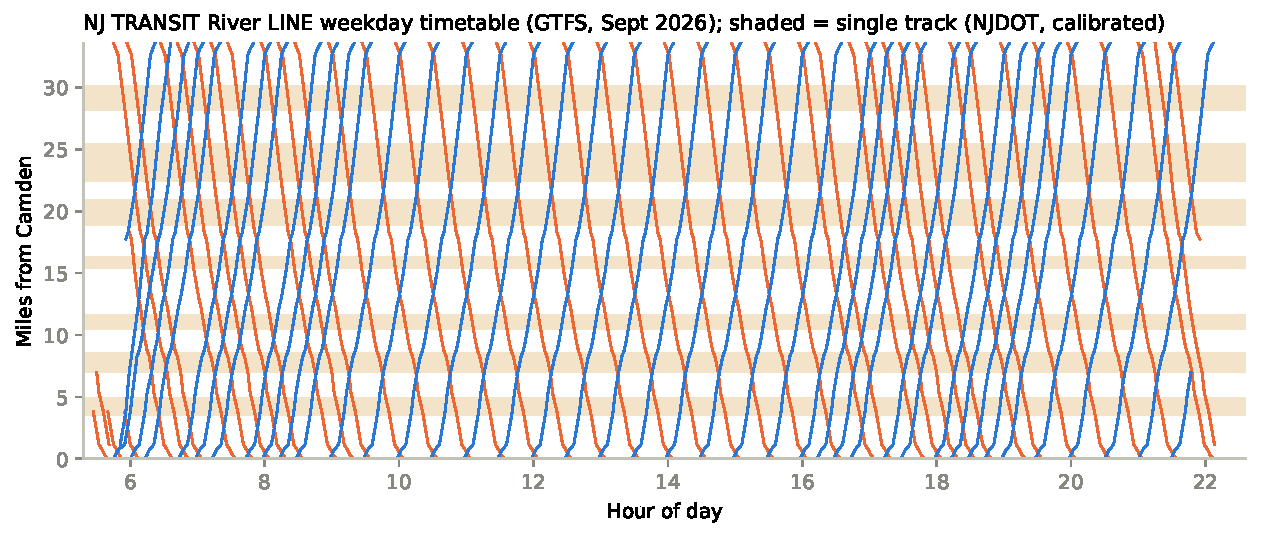
\includegraphics[width=\textwidth]{fig_gtfs_timespace.pdf}
\caption{NJ TRANSIT weekday timetable, September 2026. Blue: toward Trenton; orange: toward Camden; shaded: calibrated single track.}\label{fig:gtfs}
\end{figure}

\subsection{How many trains each headway needs (Model U)}\label{sec:resU}
With the calibrated track and $g=0.5$, Model U needs 10 trains at a 15-minute headway, 9 at 20, 8 at 21--22, 7 at 23--25 and 5 at 30 (Figure~\ref{fig:ladder}). This is the main timetable finding: \textbf{the 15/15/30 pattern is what lets NJ TRANSIT run its peak with 8 trains}; even 20-minute spacing needs a ninth. Model P confirms that no 8-train pattern exists on a 144-minute cycle; the shortest feasible cycle for 8 trains lies between 144 and 146 minutes.

\begin{figure}[ht]\centering
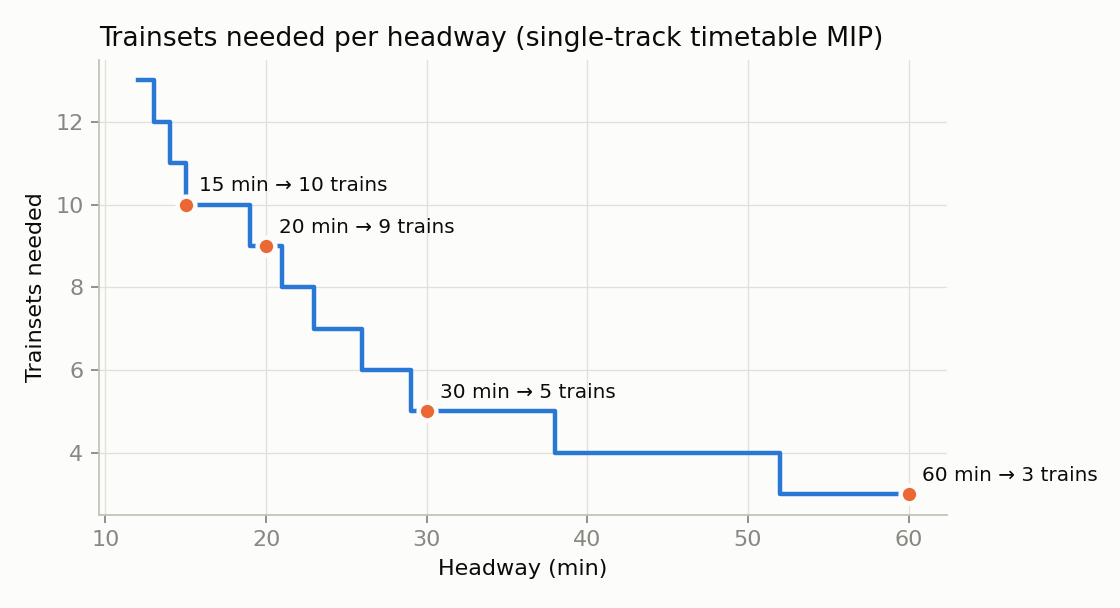
\includegraphics[width=0.7\textwidth]{fig_headway_ladder.png}
\caption{Minimum trains for each uniform headway (Model U, calibrated track, $g=0.5$).}\label{fig:ladder}
\end{figure}

\subsection{Pattern timetables T8--T3 (Model P)}\label{sec:resP}
Table~\ref{tab:tiers} summarizes the tiers. T8 uses exactly today's trains and train-hours and cuts the largest morning gap from 30 to 21 minutes toward Trenton (Figure~\ref{fig:ttcompare}). Below 8 trains the tiers degrade gracefully and, from T5 down, are almost perfectly even.

\begin{table}[ht]\centering\small
\begin{adjustbox}{max width=\linewidth}
\begin{tabular}{@{}lrrrrrr@{}}
\toprule
Timetable & Trains peak/mid & Trips & Train-hours & AM gap to Trenton, mean / max & Avg wait (min) & Conflicts \\ \midrule
NJT current & 8/6 & 87 & 109 & 17.5 / 30 & 12.9 & 1 \\
T8 & 8/6 & 88 & 109 & 18.4 / 21 & 12.9 & 0 \\
T7 & 7/6 & 80 & 99 & 21.8 / 26 & 14.0 & 0 \\
T6 & 6/5 & 69 & 86 & 25.0 / 26 & 15.5 & 0 \\
T5 & 5/5 & 62 & 77 & 30.2 / 31 & 16.0 & 0 \\
T4 & 4/4 & 48 & 60 & 37.7 / 38 & 21.1 & 0 \\
T3 & 3/3 & 37 & 46 & 51.5 / 52 & 27.2 & 0 \\
B8 & 8/6 & 83 & 109 & 19.3 / 25 & 13.5 & 0 \\
B7 & 7/6 & 76 & 100 & 22.5 / 27 & 14.6 & 0 \\
\bottomrule
\end{tabular}
\end{adjustbox}
\caption{Timetables from Model P. Gaps at Walter Rand; average wait from \eqref{eq:wait} with an assumed hourly demand profile; conflicts are opposing trips scheduled on the same single-track section.}\label{tab:tiers}
\end{table}

\begin{figure}[ht]\centering
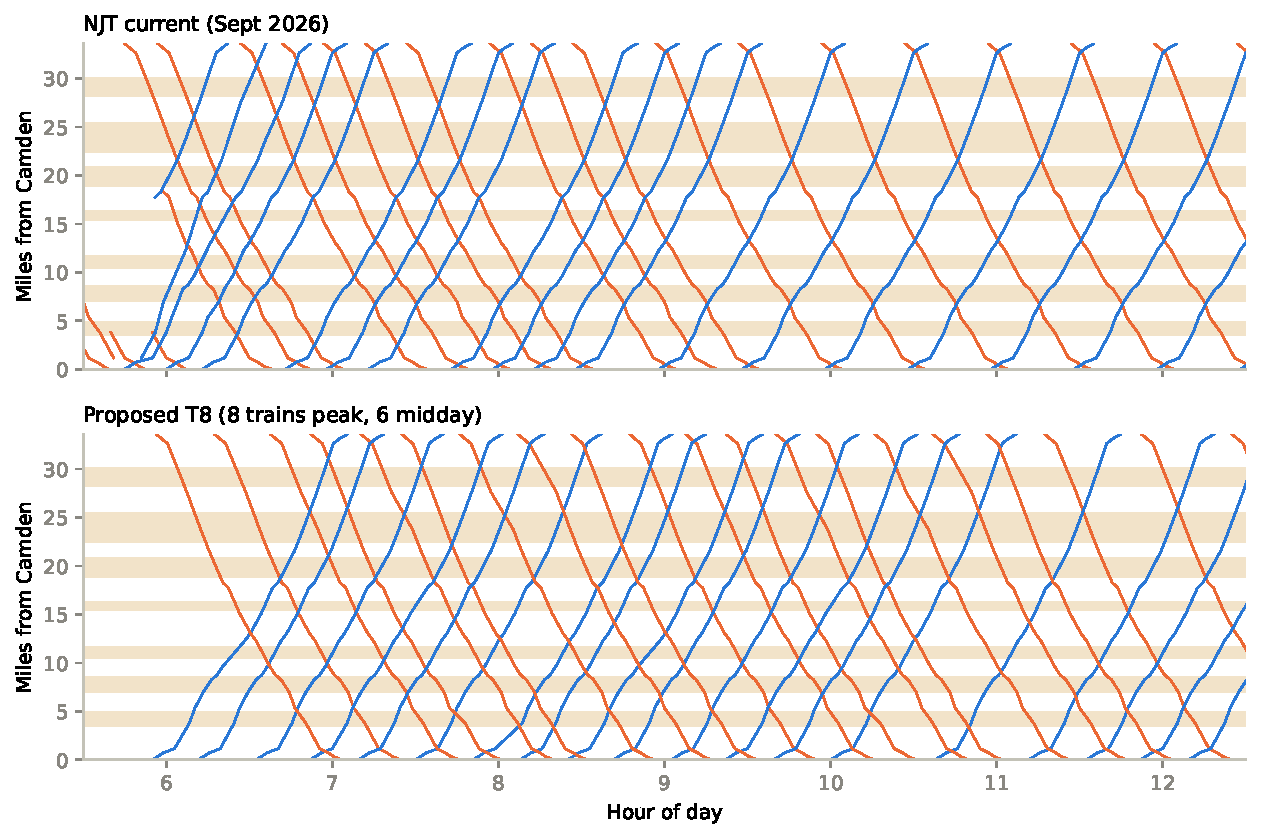
\includegraphics[width=\textwidth]{fig_tt_marey_compare.pdf}
\caption{Morning of today's timetable (top) and T8 (bottom): the same 8 trains and 150-minute cycle.}\label{fig:ttcompare}
\end{figure}

\subsection{Punctuality of each timetable (Q2)}\label{sec:resdelay}
Table~\ref{tab:delay} gives the delay-simulation results. The central finding is that \textbf{even spacing with the same trains costs punctuality}: T8 falls to 72\% on time (36\% on hot days) because 22\% of its single-track hand-offs have less than a minute to spare, against 7\% today, and its median layover drops from 9 to 6 minutes. Today's 30-minute gap works as recovery time.

\begin{table}[ht]\centering\small
\begin{adjustbox}{max width=\linewidth}
\begin{tabular}{@{}lrrrrrr@{}}
\toprule
& \multicolumn{2}{c}{Calibration run ($p_{\text{inc}}=0.211$)} & \multicolumn{2}{c}{2024--25 regime} & \multicolumn{2}{c}{2026 regime} \\
\cmidrule(lr){2-3}\cmidrule(lr){4-5}\cmidrule(lr){6-7}
Timetable & normal & hot & normal & hot & normal & hot \\ \midrule
NJT current & 84 & 60 & 83 & 60 & 93 & 83 \\
T8 & 72 & 36 & 71 & 36 & 87 & 63 \\
T7 & 76 & 47 & & & & \\
E6 (joint peak/midday) & 73 & 41 & & & & \\
S8 (holds before single track) & 74 & 43 & & & & \\
R8 (8-min layovers) & 80 & 59 & & & & \\
G8 (2-min buffers) & 80 & 55 & & & & \\
E5 (5 midday trains) & 81 & 61 & & & & \\
\textbf{B8} & \textbf{87} & \textbf{79} & \textbf{88} & \textbf{78} & \textbf{94} & \textbf{90} \\
B7 & 89 & 79 & 89 & 79 & 94 & 90 \\
W7 (summer, 7 trains) & 92 & 86 & 92 & 85 & 96 & 93 \\
\bottomrule
\end{tabular}
\end{adjustbox}
\caption{Percent of trips on time (less than 6 minutes late at the last stop), 300 simulated days each with common random numbers.}\label{tab:delay}
\end{table}

Each single-lever variant (S8, R8, G8) recovers part of T8's loss but none matches today's timetable. We therefore swept cycle, buffer and layover together (Table~\ref{tab:sweep}). The combination $C=160$, $g=2.5$, $\ell_{\min}=9$ (B8) is the most punctual 8-train pattern that keeps today's train-hours; $C=165$ needs a 32-minute gap.

\begin{table}[ht]\centering\small
\begin{adjustbox}{max width=\linewidth}
\begin{tabular}{@{}rrrrrrr@{}}
\toprule
Cycle $C$ & Buffer $g$ & Layover $\ell_{\min}$ & Train-hours & Max AM gap$^\ast$ & On time normal & On time hot \\ \midrule
150 & 1.5 & 7 & 108.7 & 30.1 & 79.5 & 54.9 \\
150 & 2.0 & 6.5 & 108.7 & 29.8 & 79.8 & 55.1 \\
155 & 1.5 & 8 & 105.6 & 30.1 & 83.6 & 69.4 \\
155 & 2.0 & 8 & 106.7 & 30.2 & 84.8 & 66.4 \\
160 & 2.0 & 8 & 107.8 & 27.0 & 84.7 & 68.8 \\
160 & 1.5 & 10 & 107.4 & 25.0 & 78.3 & 55.8 \\
165 & 2.0 & 10 & 108.0 & 32.0 & 86.1 & 75.2 \\
\textbf{160} & \textbf{2.5} & \textbf{9} & \textbf{108.7} & \textbf{30.8} & \textbf{87.1} & \textbf{79.2} \\
\bottomrule
\end{tabular}
\end{adjustbox}
\caption{Sweep of robust 8-train patterns (Model P, 6 midday trains). The bold row is B8. $^\ast$Longest morning gap in either direction.}\label{tab:sweep}
\end{table}

\begin{figure}[ht]\centering
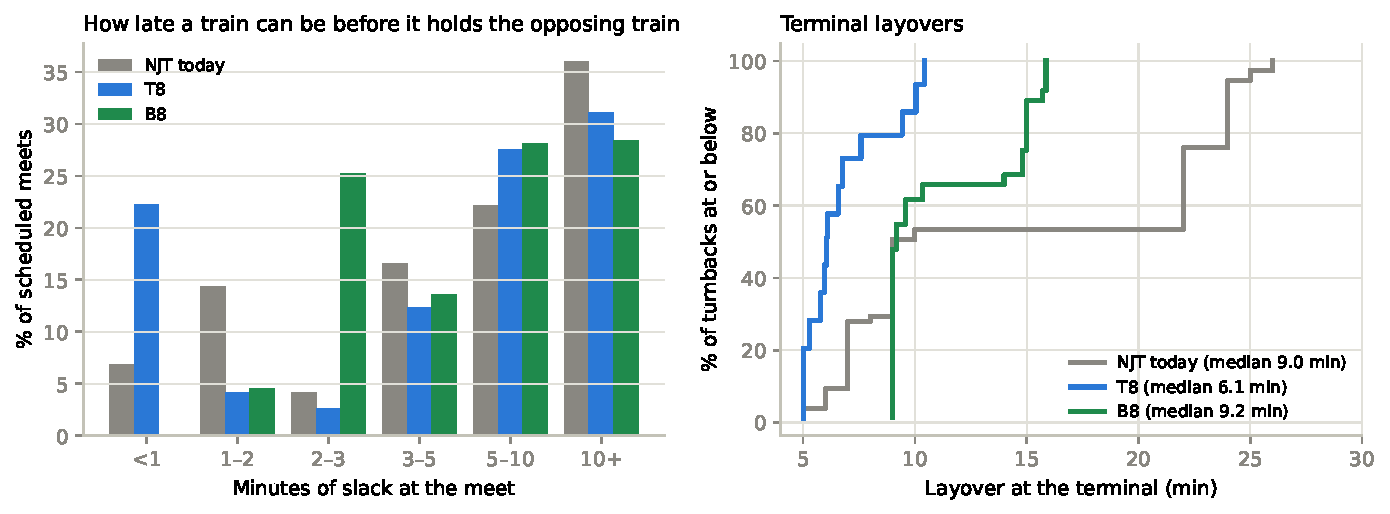
\includegraphics[width=\textwidth]{fig_prop_why.pdf}
\caption{Why: spare time at scheduled single-track meets (left) and layovers (right), by timetable.}\label{fig:why}
\end{figure}
\begin{figure}[ht]\centering
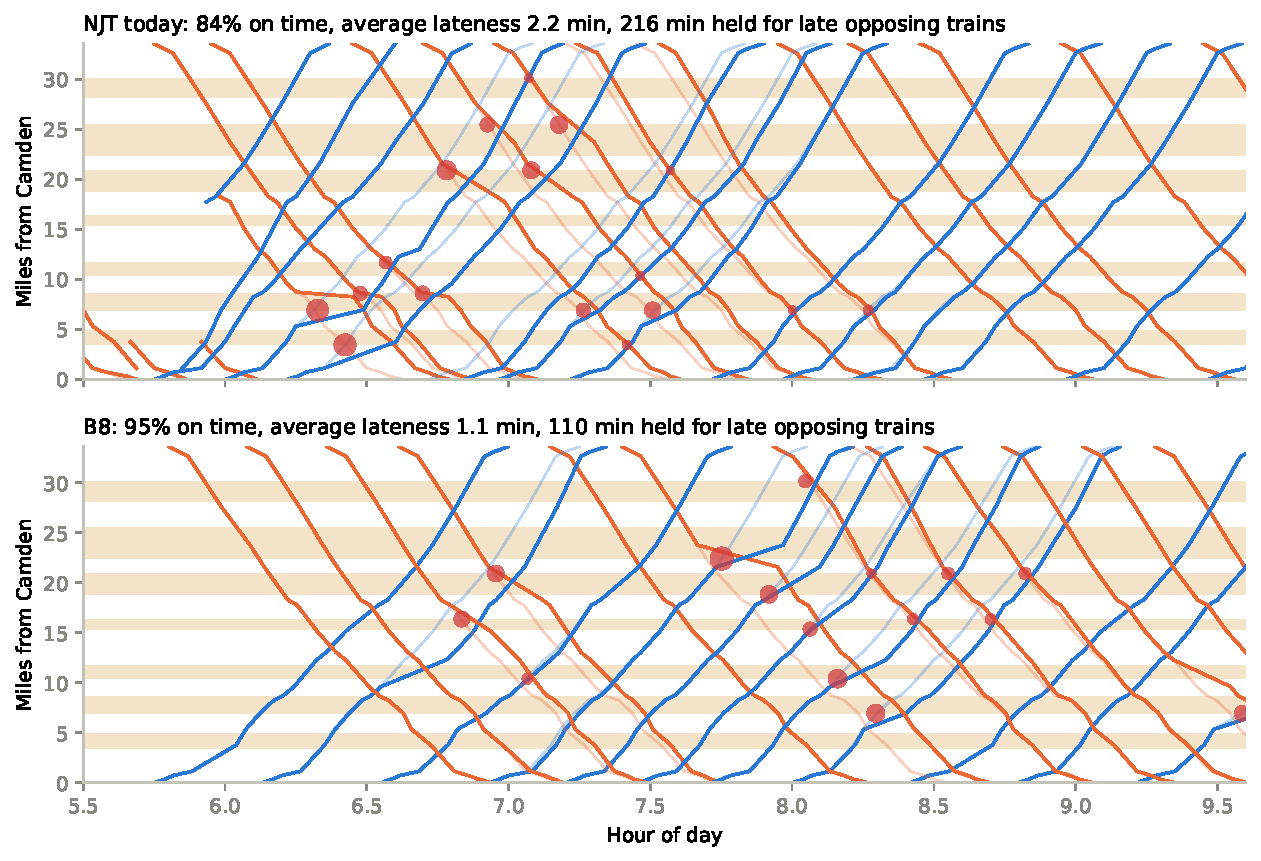
\includegraphics[width=\textwidth]{fig_prop_replay.pdf}
\caption{The same simulated morning under today's timetable (top) and B8 (bottom). Faint: schedule; solid: simulated trains; red dots: a train held at a single-track entrance (size = minutes).}\label{fig:replay}
\end{figure}

\subsection{Where and when delay builds up (Q4)}\label{sec:resbottle}
Attributing every knock-on wait in the delay simulation to the single-track section where it occurs (Figure~\ref{fig:bnsec}, Table~\ref{tab:bottle}) shows where the line bottlenecks.

\begin{table}[ht]\centering\small
\begin{adjustbox}{max width=\linewidth}
\begin{tabular}{@{}lrrrrrrr@{}}
\toprule
& \multicolumn{4}{c}{Minutes held per day (2024--25 regime)} & \multicolumn{3}{c}{Hand-offs with $<1$ min spare per day} \\
\cmidrule(lr){2-5}\cmidrule(lr){6-8}
Section & Today & B8 & T8 & B7 & Today & B8 & T8 \\ \midrule
36th Street & 30 & 23 & 58 & 16 & 1 & 0 & 23 \\
\textbf{Route 73 -- Palmyra} & \textbf{82} & 39 & 69 & 35 & \textbf{32} & 0 & 7 \\
Cinnaminson -- Riverside & 21 & 22 & 49 & 18 & 2 & 0 & 4 \\
Beverly -- Burlington South & 20 & 18 & 37 & 16 & 0 & 0 & 10 \\
Burlington -- Florence & 46 & 30 & 53 & 26 & 1 & 0 & 20 \\
Roebling & 26 & 26 & 87 & 20 & 0 & 0 & 30 \\
Bordentown -- Cass Street & 34 & 12 & 68 & 9 & 0 & 0 & 15 \\ \midrule
Total & 257 & 170 & 421 & 140 & 36 & 0 & 109 \\
On time (\%) & 82 & 88 & 69 & 88 & & & \\
\bottomrule
\end{tabular}
\end{adjustbox}
\caption{Knock-on holding by single-track section (300 simulated days) and planned hand-offs with less than one minute to spare.}\label{tab:bottle}
\end{table}

\begin{itemize}
\item \textbf{Where.} Today, the Route~73--Palmyra section accounts for 32\% of all holding. It is the slowest section to cross (about 4.5 minutes, with two stations on the single track), and today's timetable schedules 32 hand-offs a day there with less than a minute to spare. B8 removes every tight hand-off and halves the holding there; what remains reflects the section's length and dwell times, not the timetable. In T8 the bottleneck moves to Roebling, the longest section (3.1 miles).
\item \textbf{When.} About 59\% of holding happens in the two peaks (Figure~\ref{fig:bnhour}), when all eight trains are out and hand-offs come every few minutes.
\item \textbf{Fixes, in order of cost.} (1) Re-time meets to leave at least 2.5 minutes (B8); (2) a dispatching rule that swaps the meet order when the first train is several minutes late (not modeled: our simulation keeps the scheduled order, so this is an upper-bound question for future work); (3) shorter dwell at Route~73 and Palmyra; (4) if capital becomes available, extended double track through Palmyra is the first siding to study.
\end{itemize}

\begin{figure}[ht]\centering
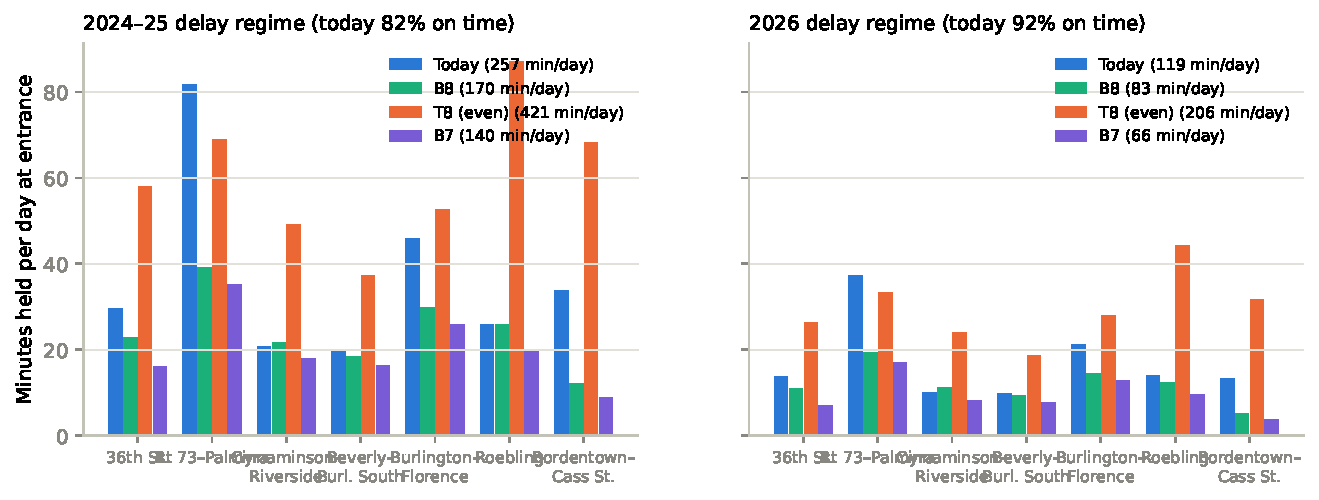
\includegraphics[width=\textwidth]{fig_bottleneck_sections.pdf}
\caption{Knock-on holding by single-track section, two delay regimes.}\label{fig:bnsec}
\end{figure}
\begin{figure}[ht]\centering
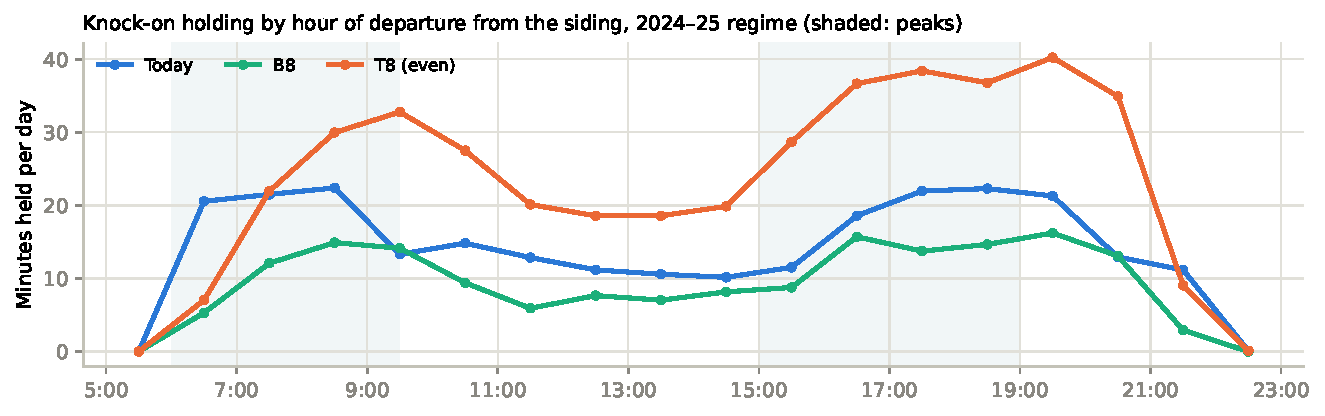
\includegraphics[width=\textwidth]{fig_bottleneck_hours.pdf}
\caption{Knock-on holding by hour of the day.}\label{fig:bnhour}
\end{figure}
\begin{figure}[ht]\centering
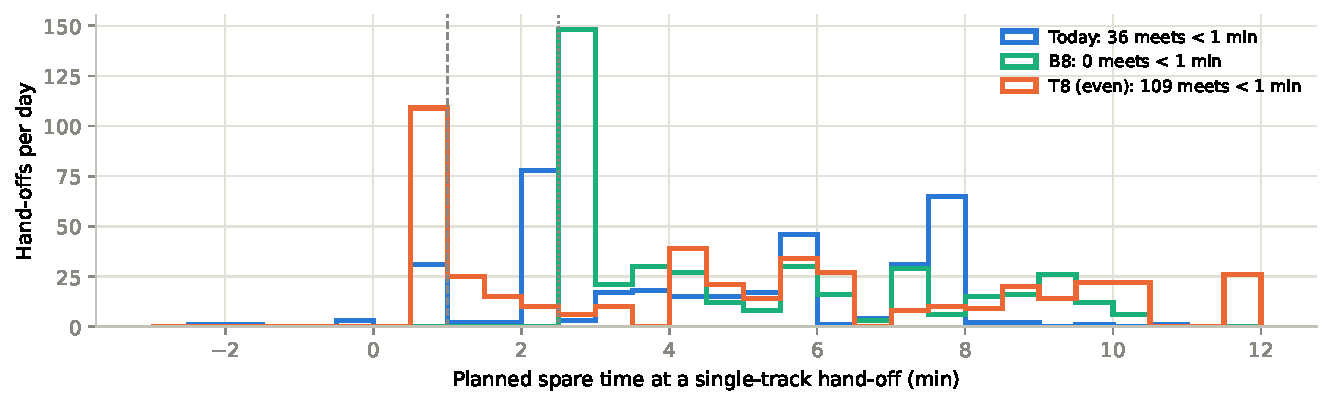
\includegraphics[width=\textwidth]{fig_meet_slack.pdf}
\caption{Distribution of planned spare time at single-track hand-offs (the time between one train leaving a section and the opposing train being due to enter it).}\label{fig:slack}
\end{figure}

\subsection{Combined results: reliable trip-miles delivered (Q3)}\label{sec:resrtd}
Table~\ref{tab:rtd} and Figure~\ref{fig:rtd} give RTD by policy and scenario over 10 simulated years.

\begin{table}[ht]\centering\small
\begin{adjustbox}{max width=\linewidth}
\begin{tabular}{@{}lrrrrr@{}}
\toprule
Policy & S1 2024--25 & S2 2026 & S3 renewed & Cancelled \% (S1/S2) & Cost (\$k/day) \\ \midrule
P1 Today's timetable & 69.4 (68--71) & 84.2 (84--85) & 85.8 & 9.7 / 2.0 & 59.4 \\
P2 B8 every day & 73.4 (71--77) & 87.5 (87--88) & 89.5 & 12.1 / 2.4 & 59.1 \\
P3 Tiers T8--T3, 1 protect & 65.4 (64--67) & 83.3 (83--84) & 84.7 & 2.2 / 2.0 & 59.1 \\
P4 Robust tiers, 1 protect & 74.4 (73--76) & 87.5 (87--88) & 89.5 & 2.4 / 1.9 & 59.1 \\
P5 Robust tiers + W7 & 73.5 (71--76) & 85.2 (85--85) & 86.8 & 2.3 / 1.8 & 57.2 \\
P6 Robust tiers, no protect & 75.3 (72--78) & 87.5 (87--88) & 89.5 & 4.0 / 2.2 & 59.1 \\
\bottomrule
\end{tabular}
\end{adjustbox}
\caption{Reliable trip-miles delivered (\%), mean and range over 10 simulated years. Cost at \$547 per train-hour.}\label{tab:rtd}
\end{table}

\begin{figure}[ht]\centering
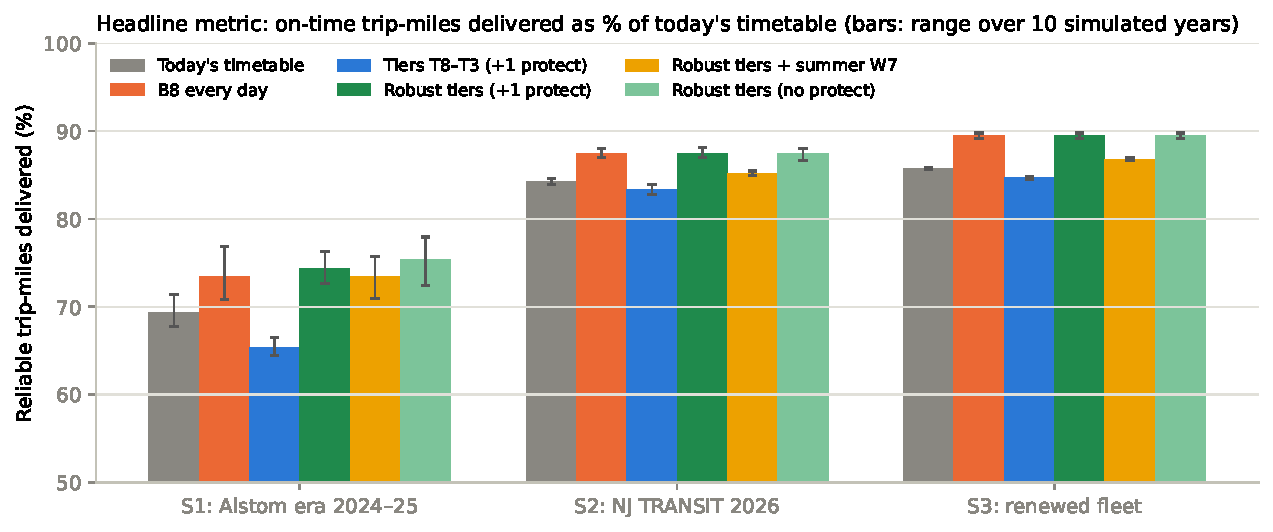
\includegraphics[width=\textwidth]{fig_rtd.pdf}
\caption{Reliable trip-miles delivered by scenario and policy (axis starts at 50\%).}\label{fig:rtd}
\end{figure}

\begin{itemize}
\item \textbf{Fleet reliability dominates.} Moving from S1 to S2 raises RTD by 13--18 points for every policy. No policy reaches 90\% even in S3.
\item \textbf{B8 is the best single schedule change}: +3--4 points in every scenario at the same cost.
\item \textbf{Daily tiers} add about one point in S1 and none in S2. Their value is predictability: on short days a smaller published timetable cancels about 4\% of its trips, against 15--52\% when today's timetable runs with whatever cars exist (Table~\ref{tab:playbook}).
\item \textbf{The original T-tiers score below today}, because T8 and T7 run late.
\end{itemize}

\paragraph{Sensitivity.} Table~\ref{tab:sens} varies repair time and MDBF. The ranking is unchanged in every case: B8-based policies lead, and the gap between S1 and S2 conditions is larger than any schedule effect.

\begin{table}[ht]\centering\small
\begin{adjustbox}{max width=\linewidth}
\begin{tabular}{@{}lrrrrrr@{}}
\toprule
Case & Cars avail. & Today & B8 & T-tiers & Robust tiers & Robust, no protect \\ \midrule
S1, repairs 8 days & 10.3 & 72.4 & 77.9 & 66.8 & 77.8 & 78.4 \\
S1 (repairs 10 days) & 8.9 & 69.4 & 73.4 & 65.4 & 74.4 & 75.3 \\
S1, repairs 12 days & 7.5 & 63.0 & 68.9 & 63.1 & 68.7 & 70.1 \\
S2, repairs 3 days & 14.7 & 84.6 & 88.0 & 83.9 & 88.0 & 88.0 \\
S2 (repairs 5 days) & 12.7 & 84.2 & 87.5 & 83.3 & 87.5 & 87.5 \\
S2, repairs 8 days & 9.9 & 80.0 & 83.9 & 79.8 & 83.3 & 84.2 \\
S2, MDBF 2{,}500 & 11.5 & 82.1 & 85.1 & 81.7 & 84.8 & 85.2 \\
\bottomrule
\end{tabular}
\end{adjustbox}
\caption{Sensitivity of RTD (\%) to repair time and failure rate.}\label{tab:sens}
\end{table}

\subsection{The 6\,am playbook}\label{sec:resplay}
\begin{table}[ht]\centering\small
\begin{adjustbox}{max width=\linewidth}
\begin{tabular}{@{}rlrrr@{}}
\toprule
Cars at 6\,am & Run & RTD & Cancelled & Today's timetable cancels \\ \midrule
9+ & B8 & 86--87\% & 3--4.5\% & 2--4\% \\
8 & B7 + 1 spare & 79\% & 4.4\% & 7.9\% \\
7 & T6 + 1 spare & 70\% & 4.3\% & 15.0\% \\
6 & T5 + 1 spare & 63\% & 4.8\% & 26.0\% \\
5 & T4 + 1 spare & 49\% & 3.6\% & 40.2\% \\
4 & T3 + 1 spare & 39\% & 4.1\% & 52.1\% \\
3 & T3, plus buses & 37\% & 10.2\% & 64.7\% \\
\bottomrule
\end{tabular}
\end{adjustbox}
\caption{Playbook, S2 conditions, summer (300 simulated days per cell). Highest RTD among plans cancelling at most 5\% of their own trips.}\label{tab:playbook}
\end{table}

\subsection{Validation}\label{sec:valid}
Table~\ref{tab:valid} compares the model with every public observation. Items marked \emph{fitted} set inputs and do not test the model.

{\small
\begin{longtable}{@{}p{3.3cm}p{4.3cm}p{4.3cm}p{3.1cm}@{}}
\caption{Model against observed data.}\label{tab:valid}\\
\toprule
Evidence & Observed & Model & Verdict \\ \midrule\endfirsthead
\toprule Evidence & Observed & Model & Verdict \\ \midrule\endhead
Miles between failures & 3{,}661 (2024--25), 3{,}568 (2026) \citep{njt_mdbf} & Input & Fitted \\
Failures per year & 267 major (435 total), NTD FY2024 \citep{ntd_breakdowns2224} & S1: about 290 & Tested: close (+8\%) \\
On time, 2024--25 & 84--87\% \citep{njtod2026,ols2027njt} & S1, today: 82\% & Tested: 2--5 points low \\
On time, 2026 & ``above 93 percent'' \citep{ols2027njt} & 93\% & Fitted \\
Worst days & 45\% (summer 2024), 56\% (2025) \citep{ols2027njt} & About 20\% with the hot-day model; 40\% without & Tested: too harsh \\
Summer 2024 shortage & 30-minute interim schedule with buses \citep{njt2024interim} & S1: fewer than 8 cars on 59\% of summer days & Tested: consistent \\
Cars in service, 2026 & 12 (March--June), 8 (July) \citep{ntd_monthly} & S2: 12.7 on average & Tested: consistent \\
Cancellations & 15 cancelled trips in July 2025 \citep{singleton2025} & S1, today: hundreds a month in summer & Not resolved \\
\bottomrule
\end{longtable}}

The model reproduces the crisis and the recovery. It overstates bad days because heat is modeled as a 6\% slowdown all day, and it cannot yet be tested on cancellations: either shortages are overstated or a reduced timetable was in force in July 2025. Train-level records would settle both.

%======================================================================
\section{Discussion}\label{sec:discussion}
\subsection{The ceiling of timetable changes}
With eight trains on this track, even spacing and punctuality pull against each other; B8 chooses punctuality and gains 3--4 RTD points. Better fleet reliability and faster repairs moved the line 15 points between S1 and S2. Even B8 on a renewed fleet reaches 89.5\%, just short of the 90\% target, so reaching it requires cutting delay at the source: fewer incidents, faster dwell, and dispatching.

\subsection{Levers beyond the timetable}
\begin{table}[ht]\centering\small
\begin{tabularx}{\textwidth}{@{}p{3.3cm}LLp{2cm}@{}}
\toprule
Lever & Evidence from our models & Data needed & Priority \\ \midrule
Fleet specification for the replacement RFP & MDBF and car count drive RTD (13--18 points) & Mostly in hand & High \\
Repair turnaround & 8$\to$3 days worth about 5 points (Table~\ref{tab:sens}) & Work orders, failure logs & Medium--high \\
Dispatching rules & Meet order is fixed in our model; swapping is untested & Train-location data & Medium \\
Running-time study & Route~73--Palmyra dominates holding & Train-location data & Medium \\
New double track & Palmyra is the first candidate & Track chart, costs & Low (short run) \\
\bottomrule
\end{tabularx}
\caption{Levers ranked by evidence and feasibility.}\label{tab:levers}
\end{table}

\subsection{Limitations}
\begin{itemize}
\item The track layout is calibrated, not surveyed; positions could shift meets by a minute.
\item Repair times are inferred; availability depends strongly on them.
\item The delay simulation keeps the scheduled meet order and models heat crudely.
\item The two simulations are combined through on-time probabilities rather than one engine; breakdown blockages and knock-on delays are not jointly simulated.
\item Ridership response to better service is not modeled.
\end{itemize}

%======================================================================
\section{Conclusions and recommendations}\label{sec:conclusions}
\begin{enumerate}
\item \textbf{Today's timetable is efficient.} Its 15/15/30 peak runs 8 trains where even spacing needs 9.
\item \textbf{Publish B8.} Same trains, same train-hours, 88\% on time in 2024--25 conditions (82\% today) and +3--4 RTD points in every scenario.
\item \textbf{Do not even out gaps without adding slack.} T8 costs 13 points of on-time performance.
\item \textbf{Adopt the 6\,am playbook for short days.} B7 and T6--T3 with a spare car keep cancellations near 4\% instead of 8--52\%.
\item \textbf{Summer timetable W7 only if heat restrictions are confirmed.}
\item \textbf{Fleet reliability is the biggest lever.} Use the models to set the replacement fleet's size and reliability requirements.
\item \textbf{Fix Route~73--Palmyra first} when looking at dispatching, dwell or infrastructure.
\end{enumerate}

\section{Future work}\label{sec:future}
\begin{itemize}
\item Re-run everything with NJ TRANSIT's hold sheets, failure logs, train-level records and track chart.
\item Test dispatching rules (meet-order swaps) in the delay simulation.
\item Optimize robustness directly (light robustness \citep{fischetti2009light}, stochastic supplements \citep{kroon2008stochastic}) instead of sweeping parameters.
\item Merge the two simulations into one engine.
\item Two-stage stochastic selection of which tiers to publish \citep{liebchen2009concept}.
\item Add ridership response and crowding to the objective.
\end{itemize}

\clearpage
\bibliographystyle{plainnat}
\bibliography{refs}

\clearpage
\appendix
\section{Model parameters}\label{app:params}
\begin{table}[ht]\centering\small
\begin{adjustbox}{max width=\linewidth}
\begin{tabular}{@{}lll@{}}
\toprule
Parameter & Value & Source / reason \\ \midrule
Running time each way & 67 min & 2026 GTFS medians \\
Clearance buffer $g$ & 0.5 min (2.5 in B8/B7) & assumption; sweep \\
Minimum layover & 5 min (9 in B8/B7) & GTFS; sweep \\
Minimum departure separation $h_{\min}$ & 6 min & assumption \\
Running-time supplement $\sigma$ & 10\% & assumption, standard practice \\
Trip / segment variability & LN, sd 0.035 / 0.12 & assumption \\
Incidents & $p_{\text{inc}}=0.210$ / 0.110; mean 6 min & fitted to 83\% / 93\% on time \\
Hot day & running time $\times$1.06; 23\% of summer days & NOAA (21 days $\ge$90\textdegree F) \\
Turnaround in delay simulation & 3 min & assumption \\
MDBF & 3{,}661 / 3{,}568 / 10{,}000 mi & NJ TRANSIT series \\
Season multiplier on MDBF & 0.85 / 1.25 / 0.65 / 1.0 & client account; literature \citep{ferranti2016heat} \\
Mean repair time & 10 / 5 days & inferred (Section~\ref{sec:valid}) \\
Long-term out of service & 3 cars & assumption \\
Rescue & dispatch 10 min, 25 mph, couple 10 min, tow 15 mph & assumption \\
Single-track blockage after a failure & 35 min & assumption \\
Cost per train-hour & \$547 & NTD FY2024 \citep{ntd_ts21} \\
\bottomrule
\end{tabular}
\end{adjustbox}
\caption{Parameters.}
\end{table}

\section{B8 and B7 patterns}
Departures within the 160-minute cycle (minutes after the first Camden departure):
\begin{itemize}
\item \textbf{B8}, Camden: 0, 25, 48, 73, 96, 112.2, 127.5, 143.0; Trenton: 76.8, 108.9, 124.0, 156.1, 172.6, 188.2, 204.7, 221.6 (mod 160). Trenton layovers 9.0--10.4 minutes.
\item \textbf{B7}, Camden: 0, 26.3, 50, 75, 98, 125, 143; Trenton: 78.2, 110.3, 126.8, 158.9, 174.0, 206.1, 223.0 (mod 160).
\end{itemize}
Full station-by-station timetables are in the Timetable Book.

\section{Software and reproducibility}
All code is in the project repository. Python 3 with pandas, NumPy, PuLP and HiGHS (open source); the fleet engine is JavaScript, run headless through Playwright.
\begin{center}\small
\begin{adjustbox}{max width=\linewidth}
\begin{tabular}{@{}ll@{}}
\toprule
File & Purpose \\ \midrule
\texttt{analysis/parse\_public.py} & GTFS parsing, running times \\
\texttt{analysis/calibrate\_track.py} & track calibration (Section~\ref{sec:calib}) \\
\texttt{src/timetable\_mip.py} & Model U \\
\texttt{analysis/timetable\_tools.py}, \texttt{proposals\_mip.py} & Model P, full-day build, blocks, conflict checker \\
\texttt{analysis/proposals\_solve.py}, \texttt{robust\_sweep.py}, \texttt{robust\_b7.py} & proposal and robust patterns \\
\texttt{analysis/timetable\_build.py} & all timetables, metrics, Timetable Book \\
\texttt{analysis/delay\_sim.py}, \texttt{delay\_eval.py}, \texttt{delay\_regimes.py} & delay simulation and calibration \\
\texttt{dashboard\_src/page\_js.js}, \texttt{jsrun.py} & fleet engine, headless runner \\
\texttt{analysis/combined\_eval.py} & RTD by scenario and policy \\
\texttt{analysis/deck\_interactive.py}, \texttt{tech\_figs.py} & bottleneck analysis and figures \\
\bottomrule
\end{tabular}
\end{adjustbox}
\end{center}
\end{document}
